%% bare_conf.tex
%% V1.3
%% 2007/01/11
%% by Michael Shell
%% See:
%% http://www.michaelshell.org/
%% for current contact information.
%%
%% This is a skeleton file demonstrating the use of IEEEtran.cls
%% (requires IEEEtran.cls version 1.7 or later) with an IEEE conference paper.
%%
%% Support sites:
%% http://www.michaelshell.org/tex/ieeetran/
%% http://www.ctan.org/tex-archive/macros/latex/contrib/IEEEtran/
%% and
%% http://www.ieee.org/

%%*************************************************************************
%% Legal Notice:
%% This code is offered as-is without any warranty either expressed or
%% implied; without even the implied warranty of MERCHANTABILITY or
%% FITNESS FOR A PARTICULAR PURPOSE!
%% User assumes all risk.
%% In no event shall IEEE or any contributor to this code be liable for
%% any damages or losses, including, but not limited to, incidental,
%% consequential, or any other damages, resulting from the use or misuse
%% of any information contained here.
%%
%% All comments are the opinions of their respective authors and are not
%% necessarily endorsed by the IEEE.
%%
%% This work is distributed under the LaTeX Project Public License (LPPL)
%% ( http://www.latex-project.org/ ) version 1.3, and may be freely used,
%% distributed and modified. A copy of the LPPL, version 1.3, is included
%% in the base LaTeX documentation of all distributions of LaTeX released
%% 2003/12/01 or later.
%% Retain all contribution notices and credits.
%% ** Modified files should be clearly indicated as such, including  **
%% ** renaming them and changing author support contact information. **
%%
%% File list of work: IEEEtran.cls, IEEEtran_HOWTO.pdf, bare_adv.tex,
%%                    bare_conf.tex, bare_jrnl.tex, bare_jrnl_compsoc.tex
%%*************************************************************************

% *** Authors should verify (and, if needed, correct) their LaTeX system  ***
% *** with the testflow diagnostic prior to trusting their LaTeX platform ***
% *** with production work. IEEE's font choices can trigger bugs that do  ***
% *** not appear when using other class files.                            ***
% The testflow support page is at:
% http://www.michaelshell.org/tex/testflow/

% Note that the a4paper option is mainly intended so that authors in
% countries using A4 can easily print to A4 and see how their papers will
% look in print - the typesetting of the document will not typically be
% affected with changes in paper size (but the bottom and side margins will).
% Use the testflow package mentioned above to verify correct handling of
% both paper sizes by the user's LaTeX system.
%
% Also note that the "draftcls" or "draftclsnofoot", not "draft", option
% should be used if it is desired that the figures are to be displayed in
% draft mode.
%
\documentclass[conference]{IEEEtran}
\usepackage{blindtext, graphicx}
% Add the compsoc option for Computer Society conferences.
%
% If IEEEtran.cls has not been installed into the LaTeX system files,
% manually specify the path to it like:
% \documentclass[conference]{../sty/IEEEtran}

% Some very useful LaTeX packages include:
% (uncomment the ones you want to load)

% *** MISC UTILITY PACKAGES ***
%
%\usepackage{ifpdf}
% Heiko Oberdiek's ifpdf.sty is very useful if you need conditional
% compilation based on whether the output is pdf or dvi.
% usage:
% \ifpdf
%   % pdf code
% \else
%   % dvi code
% \fi
% The latest version of ifpdf.sty can be obtained from:
% http://www.ctan.org/tex-archive/macros/latex/contrib/oberdiek/
% Also, note that IEEEtran.cls V1.7 and later provides a builtin
% \ifCLASSINFOpdf conditional that works the same way.
% When switching from latex to pdflatex and vice-versa, the compiler may
% have to be run twice to clear warning/error messages.

% *** CITATION PACKAGES ***
%
\usepackage{cite}
% cite.sty was written by Donald Arseneau
% V1.6 and later of IEEEtran pre-defines the format of the cite.sty package
% \cite{} output to follow that of IEEE. Loading the cite package will
% result in citation numbers being automatically sorted and properly
% "compressed/ranged". e.g., [1], [9], [2], [7], [5], [6] without using
% cite.sty will become [1], [2], [5]--[7], [9] using cite.sty. cite.sty's
% \cite will automatically add leading space, if needed. Use cite.sty's
% noadjust option (cite.sty V3.8 and later) if you want to turn this off.
% cite.sty is already installed on most LaTeX systems. Be sure and use
% version 4.0 (2003-05-27) and later if using hyperref.sty. cite.sty does
% not currently provide for hyperlinked citations.
% The latest version can be obtained at:
% http://www.ctan.org/tex-archive/macros/latex/contrib/cite/
% The documentation is contained in the cite.sty file itself.

% *** GRAPHICS RELATED PACKAGES ***
%
\ifCLASSINFOpdf
  %\usepackage[pdftex]{graphicx}
  % declare the path(s) where your graphic files are
  % \graphicspath{{../pdf/}{../jpeg/}}
  % and their extensions so you won't have to specify these with
  % every instance of \includegraphics
  %\DeclareGraphicsExtensions{.pdf,.jpeg,.png}
\else
  % or other class option (dvipsone, dvipdf, if not using dvips). graphicx
  % will default to the driver specified in the system graphics.cfg if no
  % driver is specified.
  %\usepackage[dvips]{graphicx}
  % declare the path(s) where your graphic files are
  % \graphicspath{{../eps/}}
  % and their extensions so you won't have to specify these with
  % every instance of \includegraphics
  %\DeclareGraphicsExtensions{.eps}
\fi
% graphicx was written by David Carlisle and Sebastian Rahtz. It is
% required if you want graphics, photos, etc. graphicx.sty is already
% installed on most LaTeX systems. The latest version and documentation can
% be obtained at:
% http://www.ctan.org/tex-archive/macros/latex/required/graphics/
% Another good source of documentation is "Using Imported Graphics in
% LaTeX2e" by Keith Reckdahl which can be found as epslatex.ps or
% epslatex.pdf at: http://www.ctan.org/tex-archive/info/
%
% latex, and pdflatex in dvi mode, support graphics in encapsulated
% postscript (.eps) format. pdflatex in pdf mode supports graphics
% in .pdf, .jpeg, .png and .mps (metapost) formats. Users should ensure
% that all non-photo figures use a vector format (.eps, .pdf, .mps) and
% not a bitmapped formats (.jpeg, .png). IEEE frowns on bitmapped formats
% which can result in "jaggedy"/blurry rendering of lines and letters as
% well as large increases in file sizes.
%
% You can find documentation about the pdfTeX application at:
% http://www.tug.org/applications/pdftex

% *** MATH PACKAGES ***
%
\usepackage[cmex10]{amsmath}
% A popular package from the American Mathematical Society that provides
% many useful and powerful commands for dealing with mathematics. If using
% it, be sure to load this package with the cmex10 option to ensure that
% only type 1 fonts will utilized at all point sizes. Without this option,
% it is possible that some math symbols, particularly those within
% footnotes, will be rendered in bitmap form which will result in a
% document that can not be IEEE Xplore compliant!
%
% Also, note that the amsmath package sets \interdisplaylinepenalty to 10000
% thus preventing page breaks from occurring within multiline equations. Use:
%\interdisplaylinepenalty=2500
% after loading amsmath to restore such page breaks as IEEEtran.cls normally
% does. amsmath.sty is already installed on most LaTeX systems. The latest
% version and documentation can be obtained at:
% http://www.ctan.org/tex-archive/macros/latex/required/amslatex/math/

% *** SPECIALIZED LIST PACKAGES ***
%
%\usepackage{algorithmic}
% algorithmic.sty was written by Peter Williams and Rogerio Brito.
% This package provides an algorithmic environment fo describing algorithms.
% You can use the algorithmic environment in-text or within a figure
% environment to provide for a floating algorithm. Do NOT use the algorithm
% floating environment provided by algorithm.sty (by the same authors) or
% algorithm2e.sty (by Christophe Fiorio) as IEEE does not use dedicated
% algorithm float types and packages that provide these will not provide
% correct IEEE style captions. The latest version and documentation of
% algorithmic.sty can be obtained at:
% http://www.ctan.org/tex-archive/macros/latex/contrib/algorithms/
% There is also a support site at:
% http://algorithms.berlios.de/index.html
% Also of interest may be the (relatively newer and more customizable)
% algorithmicx.sty package by Szasz Janos:
% http://www.ctan.org/tex-archive/macros/latex/contrib/algorithmicx/

% *** ALIGNMENT PACKAGES ***
%
%\usepackage{array}
% Frank Mittelbach's and David Carlisle's array.sty patches and improves
% the standard LaTeX2e array and tabular environments to provide better
% appearance and additional user controls. As the default LaTeX2e table
% generation code is lacking to the point of almost being broken with
% respect to the quality of the end results, all users are strongly
% advised to use an enhanced (at the very least that provided by array.sty)
% set of table tools. array.sty is already installed on most systems. The
% latest version and documentation can be obtained at:
% http://www.ctan.org/tex-archive/macros/latex/required/tools/

%\usepackage{mdwmath}
%\usepackage{mdwtab}
% Also highly recommended is Mark Wooding's extremely powerful MDW tools,
% especially mdwmath.sty and mdwtab.sty which are used to format equations
% and tables, respectively. The MDWtools set is already installed on most
% LaTeX systems. The lastest version and documentation is available at:
% http://www.ctan.org/tex-archive/macros/latex/contrib/mdwtools/

% IEEEtran contains the IEEEeqnarray family of commands that can be used to
% generate multiline equations as well as matrices, tables, etc., of high
% quality.

%\usepackage{eqparbox}
% Also of notable interest is Scott Pakin's eqparbox package for creating
% (automatically sized) equal width boxes - aka "natural width parboxes".
% Available at:
% http://www.ctan.org/tex-archive/macros/latex/contrib/eqparbox/

% *** SUBFIGURE PACKAGES ***
%\usepackage[tight,footnotesize]{subfigure}
% subfigure.sty was written by Steven Douglas Cochran. This package makes it
% easy to put subfigures in your figures. e.g., "Figure 1a and 1b". For IEEE
% work, it is a good idea to load it with the tight package option to reduce
% the amount of white space around the subfigures. subfigure.sty is already
% installed on most LaTeX systems. The latest version and documentation can
% be obtained at:
% http://www.ctan.org/tex-archive/obsolete/macros/latex/contrib/subfigure/
% subfigure.sty has been superceeded by subfig.sty.

%\usepackage[caption=false]{caption}
%\usepackage[font=footnotesize]{subfig}
% subfig.sty, also written by Steven Douglas Cochran, is the modern
% replacement for subfigure.sty. However, subfig.sty requires and
% automatically loads Axel Sommerfeldt's caption.sty which will override
% IEEEtran.cls handling of captions and this will result in nonIEEE style
% figure/table captions. To prevent this problem, be sure and preload
% caption.sty with its "caption=false" package option. This is will preserve
% IEEEtran.cls handing of captions. Version 1.3 (2005/06/28) and later
% (recommended due to many improvements over 1.2) of subfig.sty supports
% the caption=false option directly:
%\usepackage[caption=false,font=footnotesize]{subfig}
%
% The latest version and documentation can be obtained at:
% http://www.ctan.org/tex-archive/macros/latex/contrib/subfig/
% The latest version and documentation of caption.sty can be obtained at:
% http://www.ctan.org/tex-archive/macros/latex/contrib/caption/

% *** FLOAT PACKAGES ***
%
%\usepackage{fixltx2e}
% fixltx2e, the successor to the earlier fix2col.sty, was written by
% Frank Mittelbach and David Carlisle. This package corrects a few problems
% in the LaTeX2e kernel, the most notable of which is that in current
% LaTeX2e releases, the ordering of single and double column floats is not
% guaranteed to be preserved. Thus, an unpatched LaTeX2e can allow a
% single column figure to be placed prior to an earlier double column
% figure. The latest version and documentation can be found at:
% http://www.ctan.org/tex-archive/macros/latex/base/

%\usepackage{stfloats}
% stfloats.sty was written by Sigitas Tolusis. This package gives LaTeX2e
% the ability to do double column floats at the bottom of the page as well
% as the top. (e.g., "\begin{figure*}[!b]" is not normally possible in
% LaTeX2e). It also provides a command:
%\fnbelowfloat
% to enable the placement of footnotes below bottom floats (the standard
% LaTeX2e kernel puts them above bottom floats). This is an invasive package
% which rewrites many portions of the LaTeX2e float routines. It may not work
% with other packages that modify the LaTeX2e float routines. The latest
% version and documentation can be obtained at:
% http://www.ctan.org/tex-archive/macros/latex/contrib/sttools/
% Documentation is contained in the stfloats.sty comments as well as in the
% presfull.pdf file. Do not use the stfloats baselinefloat ability as IEEE
% does not allow \baselineskip to stretch. Authors submitting work to the
% IEEE should note that IEEE rarely uses double column equations and
% that authors should try to avoid such use. Do not be tempted to use the
% cuted.sty or midfloat.sty packages (also by Sigitas Tolusis) as IEEE does
% not format its papers in such ways.

% *** PDF, URL AND HYPERLINK PACKAGES ***
%
\usepackage{url}
% url.sty was written by Donald Arseneau. It provides better support for
% handling and breaking URLs. url.sty is already installed on most LaTeX
% systems. The latest version can be obtained at:
% http://www.ctan.org/tex-archive/macros/latex/contrib/misc/
% Read the url.sty source comments for usage information. Basically,
% \url{my_url_here}.


% *** Do not adjust lengths that control margins, column widths, etc. ***
% *** Do not use packages that alter fonts (such as pslatex).         ***
% There should be no need to do such things with IEEEtran.cls V1.6 and later.
% (Unless specifically asked to do so by the journal or conference you plan
% to submit to, of course. )
\usepackage{amssymb}
% correct bad hyphenation here
\hyphenation{op-tical net-works semi-conduc-tor}
\usepackage[bookmarks, colorlinks=false, pdfborder={0 0 0},
            pdftitle={Security Implementation using Biometric},
            pdfauthor={Shrimadhav U K _ B130253CS}, pdfsubject={CS4089_Project},
            pdfkeywords={r,e,l,e,v,a,n,t,k,e,y,w,o,r,d,s}]{hyperref} %for creating links in the pdf version and other additional pdf attributes, no effect on the printed document
\begin{document}
%
% paper title
% can use linebreaks \\ within to get better formatting as desired
\title{Security Implementation using Biometric}

% author names and affiliations
% use a multiple column layout for up to three different
% affiliations
\author{\IEEEauthorblockN{Shrimadhav U K}
        \IEEEauthorblockA{\\
                          Guided by: \textbf{Dr. Vinod Pathari}\\ \\
                          December 2, 2016\\
      }}


% conference papers do not typically use \thanks and this command
% is locked out in conference mode. If really needed, such as for
% the acknowledgment of grants, issue a \IEEEoverridecommandlockouts
% after \documentclass

% use for special paper notices
%\IEEEspecialpapernotice{(Invited Paper)}

% make the title area
\maketitle

\begin{abstract}
%\boldmath
The project aims to develop a biometric security system, which can protect the
user's device from unauthorized or unauthenticated access. The
idea is inspired from Microsoft Windows Hello and Google Now, which allows us
to speak our mind and the machine does it, through the profound
advancement in machine learning and artificial intelligence. This project aims
to implement an application which can recognize the face and the voice of
the user, and accordingly allow or deny access to the system.
\end{abstract}

% IEEEtran.cls defaults to using nonbold math in the Abstract.
% This preserves the distinction between vectors and scalars. However,
% if the journal you are submitting to favors bold math in the abstract,
% then you can use LaTeX's standard command \boldmath at the very start
% of the abstract to achieve this. Many IEEE journals frown on math
% in the abstract anyway.

% Note that keywords are not normally used for peerreview papers.
\begin{IEEEkeywords}
CMUSphinx, OpenCV, Real time, biometric, Face Recognition, PCA, eigenfaces,
Yale Face DataBase, Principle Component Analysis,
%IEEEtran, journal, \LaTeX, paper, template.
\end{IEEEkeywords}

% For peer review papers, you can put extra information on the cover
% page as needed:
% \ifCLASSOPTIONpeerreview
% \begin{center} \bfseries EDICS Category: 3-BBND \end{center}
% \fi
%
% For peerreview papers, this IEEEtran command inserts a page break and
% creates the second title. It will be ignored for other modes.
\IEEEpeerreviewmaketitle

\section{Introduction}
Biometric Security is gaining more and more attention recently. This project
attempts to implement an application which can take the voice input from a
microphone, face input from a camera, and verify the authenticity of the user
accessing the system. \\

\section{Motivation}
Human beings have reached a stage where it is no longer convenient to type the
password when they want to be authenticated. This was the basic motivation of
this project, i.e., to replace the password input using a keyboard, and instead
ask the user to smile in front of their personal computer, and talk interactively
to it. Then that personal computer unlocks, if it recognizes the integrity of
the user. \\
Currently, no fool-proof solution exists which attempts to do both these tasks.
There exists individual solutions for each of these individual tasks. But, these
solutions are proprietary and requires specific licenses to use the offered
services. \\

\section{Problem Statement}
To design a security system for GNU/Linux operating system using biometric
of the user, i.e., the face and the voice of the user, that would replace the
traditional password input using a keyboard. \\

\section{Related Works}
\begin{enumerate}
  \item Google Now \url{https://www.google.com/search/about/learn-more/now/}
  \item Microsoft Windows Hello \url{https://support.microsoft.com/en-in/help/17215/windows-10-what-is-hello}
\end{enumerate}

\section{High Level Design}
\begin{enumerate}
  \item Design a function which takes the user voice through the microphone,
        and the name of the user and returns True or False, accordingly.
  \item Design a function which takes an image of the user, using the camera,
        and the name of the user and returns True or False, accordingly.
  \item Finally, design a system which unifies the functions designed above.
        The system should be able:
        \begin{itemize}
          \item to override the default login screen in a GNU/Linux system.
          \item to ensure the integrity of the confidential details created
                using the above functions.
        \end{itemize}
\end{enumerate}

\section{Literature Survey}

\subsection{Background and Related Work}
Much of the work in computer recognition of faces have been approached by
characterizing a face by a set of geometric parameters and performing pattern
recognition based on the parameters. \\
Kanade's face identification system \cite{Kanade1973} was the first system in which all
steps of the recognition process were automated, using a top-down control strategy
directed by a generic model of expected feature characteristics. His system calculated
a set of facial parameters from a single face image and used a pattern classification
technique to match the face from a known set. This approach was a statistical
based approach, which depended primarily on local histogram analysis and absolute
gray-scale values. \\

\subsection{The EigenFace Approach}
Much of the previous work on automated face recognition has ignored the issue of
just what aspects of the face stimulus are important for identification.
This suggested that an information theory approach of encoding and decoding
face images may give insight into the information content of face images,
emphasizing the significant local and global features. Such features may or may not
be directly related to our intuitive notion of face features such as the eyes, nose,
lips, and hair. \\
In the language of information theory, the relevant information in a face image
should be extracted, encode it as efficiently as possible, and compare one face
encoding with a database of models encoded similarly. \\
A simple approach to extracting the information contained in an image of a face
is to somehow capture the variation in a collection of face images, independent
of any judgment of features, and use this information to encode and compare
individual face images. \\
In mathematical terms, we wish to find the principal components of the distribution of
faces, or the eigenvectors of the covariance matrix of the set of face images,
treating an image as a vector in a very high dimensional space. The eigenvectors
are ordered, each one accounting for a different amount of the variation among the face
images. \\
These eigenvectors can be thought of as a set of features that together characterize
the variation between face images. Each image location contributes more or less
to each eigenvector, so that the eigenvector is displayed as a sort of ghostly
face, which is called an eigenface (see Figure \ref{fig:meigenface}). \\
The approach to face recognition using the eigenface approach involves the
following initiation operations: \\
\begin{enumerate}
  \item Acquire an initial set of characteristic face images (the training set). \\
        This set should include a number of images for each person, with some
        variation in expression and in the lighting. \\
        (say \textbf{4} images of \textbf{10} people, so \textbf{M = 40}.)
  \item Calculate the eigenfaces from the training set, keeping only the M images
        that correspond to the highest eigenvalues. \\
        These M images define the \textit{face space}. As new faces are experienced,
        the eigenfaces can be updated or re-calculated.
        \begin{enumerate}
          \item Calculate the (M x M) matrix L, find it's eigenvectors and
                eigenvalues, and choose the M' eigenvectors with the highest
                associated eigenvalues. \\
                (Let $ M' = 10 $ in this example.)
          \item Combine the normalized training set of images (according to
                equation (\ref{eq:six})) to produce the (say, $ M' = 10 $) eigenfaces $ u_{k} $. \\
                \begin{equation} \label{eq:six}
                  u_{l} = \sum_{k = 1}^{M} v_{lk}\Phi_{k} \hspace{10 mm}, l = 1,2,\ldots,M
                \end{equation}
          \item For each known individual, calculate the class vector $ \Omega_{k} $
                by averaging the eigenface pattern vectors $ \Omega $ (from equation (\ref{eq:eight}))
                calculated from the original images (four, in this example) of the individual. \\
                \begin{equation} \label{eq:eight}
                  \epsilon_{k}^{2} = || (\Omega - \Omega_{k}) ||^{2}
                \end{equation}
                Choose a threshold $ \theta_{\epsilon} $ that defines the maximum
                allowable distance from any face class, and a threshold $ \theta_{\epsilon} $
                that defines the maximum allowable distance from face space.
                (according to equation (\ref{eq:nine})) \\
                \begin{equation} \label{eq:nine}
                  \epsilon^{2} = || (\Phi - \Phi_{f}) ||^{2}
                \end{equation}
          \item For each new face image to be identified, calculate it's pattern
                vector $ \Omega $, the distance $ \epsilon_{i} $ to each known
                class, and the distance $ \epsilon $ to face space. \\
                If the minimum distance $ \epsilon_{k} < \Theta_{\epsilon} $
                and the distance $ \epsilon < \Theta_{\epsilon} $, classify the
                input face as the individual associated with the class vector
                $ \Omega_{k} $. \\
                If the minimum distance $ \epsilon_{k} > \Theta_{\epsilon} $ but
                distance $ \epsilon < \Theta_{\epsilon} $, Then the image may be
                classified as unknown, and optionally used to begin a new face class.
        \end{enumerate}
  \item If the new image is classified as a known individual, this image may be added
        to the original set of familiar face images, and the eigenfaces may be recalculated
        (steps 1-2). This gives the opportunity to modify the face space as the
        system encounters more instances of known faces.
  \item Calculate the corresponding in M-dimensional weight space for each known
        individual, by projecting the face images onto the face space.
\end{enumerate}
The above initialization operations can be performed from time to time whenever
there is free excess computational capacity, available in the system. \\
Having initialized the system, the following steps are then used to recognize
new face images: \\
\begin{enumerate}
  \item Calculate a set of weights based on the input image and the M eigenfaces
        by projecting the input image onto each of the eigenfaces.
  \item Determine if the image is a face (whether known or unknown) by checking
        to see if the image is sufficiently close to face space.
  \item If it is a face, classify the weight pattern as either a known person or
        as unknown.
  \item Update the eigenfaces and/or weight pattern.
  \item If the same unknown face is seen several times, calculate its characteristic
        weight pattern and incorporate into the known faces.
\end{enumerate}

\begin{figure}[!t]
\centering
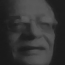
\includegraphics[width=1.5in]{./gulzar.png}
% where an .eps filename suffix will be assumed under latex,
% and a .pdf suffix will be assumed for pdflatex; or what has been declared
% via \DeclareGraphicsExtensions.
\caption{Mean Eigen Face}
\label{fig:meigenface}
\end{figure}

In the prototype implemented using the eigenfaces approach, calculation of the
eigenfaces is done as part of the training process. \\
The recognition, using the eigenfaces approach, takes about 90 seconds
implemented in Python on an Intel Core i5, using face images of size 132 x 132. \\

\subsection{The Local Binary Pattern Histogram Approach}
It is observed that if the above program is run without any alterations,
trained with a specific person, and another untrained face is introduced,
then it will be recognized as the trained person. \\
The methods to improve the accuracy of the Face Recognizer have been made more
stringent. The threshold used to control unknown faces, in the case of the
EigenFaceRecognizer, from the calculated distance can be adjusted to allow better
accuracy. A default of 2000 is used but by increasing this to 5000, for example,
will mean it will be less likely to allow a false match. \\

\subsection{Principle Component Analysis}
The EigenFaceRecognizer class applies PCA on each image, the results of which will
be an array of Eigen values that a neural network can be trained to recognize. \\
The LBPHFaceRecognizer uses Local Binary Patterns (LBP) to create a feature vector
using a Support Vector Machine or some other machine learning algorithm. \\

\subsection{The Local Binary Pattern Histogram Classifier}
The LBPH recognizer takes five variables: \\
\begin{description}
  \item[\textbf{radius}] \quad
  The radius used for building the Circular Local Binary Pattern.

  \item[\textbf{neighbors}] \quad
  The number of sample points to build a Circular Local Binary Pattern from.
  A value suggested by OpenCV documentation is eight sample points.
  The more the number of sample points, higher will be the computational cost.

  \item[\textbf{grid\_x}] \quad
  The number of cells in the horizontal direction.
  Eight is a common value used in publications.
  The more cells, the finer the grid, the higher the dimensionality of the
  resulting feature vector.

  \item[\textbf{grid\_y}] \quad
  The number of cells in the vertical direction.
  Eight is a common value used in publications.
  The more cells, the finer the grid, the higher the dimensionality of the
  resulting feature vector.

  \item[\textbf{threshold}] \quad
  The threshold applied in the prediction.
  If the distance to the nearest neighbor is larger than the threshold,
  the method returns \textbf{-1}.
\end{description}

\begin{figure}[!t]
\centering
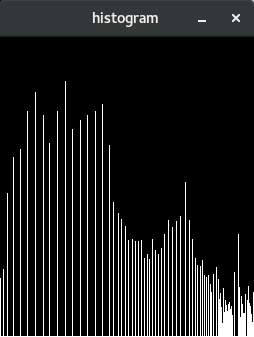
\includegraphics[width=1.5in]{./histogram.png}
% where an .eps filename suffix will be assumed under latex,
% and a .pdf suffix will be assumed for pdflatex; or what has been declared
% via \DeclareGraphicsExtensions.
\caption{Local Binary Pattern}
\label{fig:lbph}
\end{figure}

In the prototype implemented using the LBPH Approach (see Figure (\ref{fig:lbph})), calculation of the
LBP is done as part of the training process. \\
The recognition, using the LBPH approach, takes about 30 milliseconds
implemented in Python on an Intel Core i5, using face images of size 132 x 132. \\

\subsection{Background and Related Work}
Speaker recognition is the identification of the person who is speaking by
characteristics of their voices (voice biometrics), also called voice recognition. \\
Speech is a kind of complicated signal produced as a result of several transformations
occuring at different levels: semantic, linguistic and acoustic. Differences in these transformations may lead to differences in the acoustic properties of signals. The recognizability of speaker can be affected not only by the linguistic message but also the age, health, emotional state and effort level of the speaker. \\
Background noise and performance of recording device also interfere the classification process. \\
Speaker recognition is an important part of Human-Computer Interaction (HCI). As the trend of employing wearable computer reveals, Voice User Interface (VUI) has been a vital part of such computer. As these devicesare particularly small, they are more likely to lose and be stolen. In these scenarios, speaker recognition is not only a good HCI, but also a combination of seamless interaction with computer and security guard when the device is lost. The need of personal identity validation will become more acute in the future. Telephone banking and Telephone reservation services will develop rapidly when secure means of authentication are available. \\

\subsection{Algorithm Used}
\begin{enumerate}
  \item An utterance of a user is collected during the enrollment procedure.
  \item Voice Activity Detection is performed: Signals must be first filtered to rule out the silence part, otherwise the training might be seriously biased.
  \item Feature Extraction
    \begin{itemize}
      \item Mel-Frequency Cepstral Coefficient (MFCC) is a representation of the short term power spectrum of a sound, based on a linear cosine transform of a log power spectrum on a non-linear mel-scale of frequency . MFCC is the most widely used features in Automatic Speech Recognition, and it can also be applied to speaker recognition task. The process to extract MFCC feature is demonstrated in Figure \ref{fig:MFCC_fig_one}. \\
      \begin{figure}[!t]
      \centering
      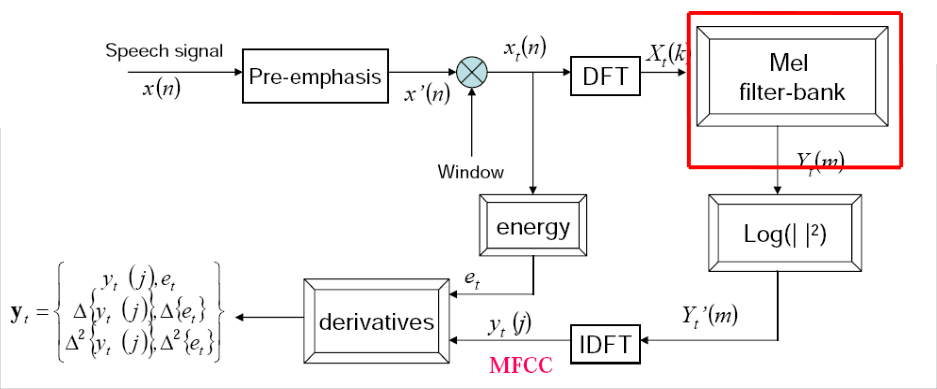
\includegraphics[width=2.5in]{./MFCC-mel-filterbank.png}
      % where an .eps filename suffix will be assumed under latex,
      % and a .pdf suffix will be assumed for pdflatex; or what has been declared
      % via \DeclareGraphicsExtensions.
      \caption{MFCC Feature Extraction Process}
      \label{fig:MFCC_fig_one}
      \end{figure}
      \\
      \item Linear Predictive Coding (LPC) is a tool used in audio signal processing and speech processing for representing the spectral envelope of a digital signal of speech in compressed form, using the information of a Linear predictive Model. \\
      The basic assumption in LPC is that, the n th signal is a linear combination of the previous p signals. Therefore, to estimate the coefficients ai, we have to minimize the squared error. This optimization can be done by Levinson-Durbin algorithm.
    \end{itemize}
  \item Gaussian Mixture Model (GMM) is used in acoustic learning task such as speaker recognition, since it describes the varied distribution of all the feature vectors. Therefore, GMM is merely a weighted combination of multivariate Gaussian distribution which assumes feature vectors are independent. We use diagonal covariance since the dimensions of the feature vector is independent to each other. GMM can describe the distribution of feature vector with several clusters, as shown in Figure \ref{fig:GMM_fig_one}. \\
  \begin{figure}[!t]
  \centering
  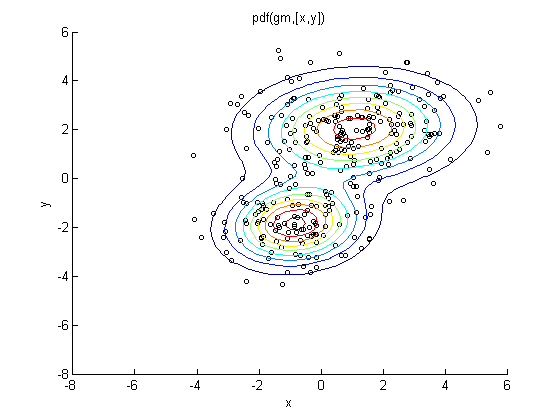
\includegraphics[width=2.5in]{./gmm.png}
  % where an .eps filename suffix will be assumed under latex,
  % and a .pdf suffix will be assumed for pdflatex; or what has been declared
  % via \DeclareGraphicsExtensions.
  \caption{A Two Dimensional GMM with Two Components}
  \label{fig:GMM_fig_one}
  \end{figure}
  \\
  After training, the model can give the score of fitness for every input feature vector, measuring the probability that the vector belongs to this model. Therefore in the task of speaker recognition, we can train a GMM for every speaker. Then for a input signal, we extract lists of feature vectors for it, and calculate the overall likelihood that the vector belongs to each model. The speaker whose model fits the input best will be chosen as the answer. \\
  Moreover, an enhancement has been done to the original GMM method. The training of GMM first requires a random initialization of the means of all the components. However, we can first use K-means algorithm to perform a clustering to all the vectors, then use the clustered centers to initialize the training of GMM. This enhancement can speed up the training and also give a better training result.
  \item Joint Factor Analysis (JFA) is a typical method which behave very well in classification problems, due to its ability to account for different types of variability in training data. Within all the factor analysis methods, JFA was proved to outperform other methods in the task of speaker recognition. \\  JFA models the user by supervector, i.e., a C x F dimension vector, where C is the number of components in the Universal Background Model, trained by GMM on all the training data, and F is the dimension of the acoustic feature vector. The supervector of an utterance is obtained by concatenating all the C means vectors in the trained GMM model.
\end{enumerate}

\section{Work Plan}
\begin{enumerate}
  \item Learn how the GNU/Linux login screen works, and possible ways to overwrite it.
  \item Implement the custom application as the new login screen in GNU/Linux system.
  \item Discover the ways to improve the application, and document the challenges
        faced during the implementation phase.
\end{enumerate}

\section{Conclusion}
In this project, I have implemented a face recognition based biometric
security system. It also demonstrates the various capabilities of image recognition
from video sequences. \\
I have also implemented a voice recognition based biometric security system. It demonstrates
the capabilities of speech based recognition from audio sequences. \\
However, several aspects remain to be researched and extended.
For instance, since face to face meeting encompasses several modalities, such as
speech and gesture, these capabilities need to researched and implemented. \\ 

%\subsection{Subsection Heading Here}
%\blindtext

% needed in second column of first page if using \IEEEpubid
%\IEEEpubidadjcol

% An example of a floating figure using the graphicx package.
% Note that \label must occur AFTER (or within) \caption.
% For figures, \caption should occur after the \includegraphics.
% Note that IEEEtran v1.7 and later has special internal code that
% is designed to preserve the operation of \label within \caption
% even when the captionsoff option is in effect. However, because
% of issues like this, it may be the safest practice to put all your
% \label just after \caption rather than within \caption{}.
%
% Reminder: the "draftcls" or "draftclsnofoot", not "draft", class
% option should be used if it is desired that the figures are to be
% displayed while in draft mode.
%
%\begin{figure}[!t]
%\centering
%\includegraphics[width=2.5in]{myfigure}
% where an .eps filename suffix will be assumed under latex,
% and a .pdf suffix will be assumed for pdflatex; or what has been declared
% via \DeclareGraphicsExtensions.
%\caption{Simulation Results}
%\label{fig_sim}
%\end{figure}

% Note that IEEE typically puts floats only at the top, even when this
% results in a large percentage of a column being occupied by floats.

% An example of a double column floating figure using two subfigures.
% (The subfig.sty package must be loaded for this to work.)
% The subfigure \label commands are set within each subfloat command, the
% \label for the overall figure must come after \caption.
% \hfil must be used as a separator to get equal spacing.
% The subfigure.sty package works much the same way, except \subfigure is
% used instead of \subfloat.
%
%\begin{figure*}[!t]
%\centerline{\subfloat[Case I]\includegraphics[width=2.5in]{subfigcase1}%
%\label{fig_first_case}}
%\hfil
%\subfloat[Case II]{\includegraphics[width=2.5in]{subfigcase2}%
%\label{fig_second_case}}}
%\caption{Simulation results}
%\label{fig_sim}
%\end{figure*}
%
% Note that often IEEE papers with subfigures do not employ subfigure
% captions (using the optional argument to \subfloat), but instead will
% reference/describe all of them (a), (b), etc., within the main caption.

% An example of a floating table. Note that, for IEEE style tables, the
% \caption command should come BEFORE the table. Table text will default to
% \footnotesize as IEEE normally uses this smaller font for tables.
% The \label must come after \caption as always.
%
%\begin{table}[!t]
%% increase table row spacing, adjust to taste
%\renewcommand{\arraystretch}{1.3}
% if using array.sty, it might be a good idea to tweak the value of
% \extrarowheight as needed to properly center the text within the cells
%\caption{An Example of a Table}
%\label{table_example}
%\centering
%% Some packages, such as MDW tools, offer better commands for making tables
%% than the plain LaTeX2e tabular which is used here.
%\begin{tabular}{|c||c|}
%\hline
%One & Two\\
%\hline
%Three & Four\\
%\hline
%\end{tabular}
%\end{table}

% Note that IEEE does not put floats in the very first column - or typically
% anywhere on the first page for that matter. Also, in-text middle ("here")
% positioning is not used. Most IEEE journals use top floats exclusively.
% Note that, LaTeX2e, unlike IEEE journals, places footnotes above bottom
% floats. This can be corrected via the \fnbelowfloat command of the
% stfloats package.

% if have a single appendix:
%\appendix[Proof of the Zonklar Equations]
% or
%\appendix  % for no appendix heading
% do not use \section anymore after \appendix, only \section*
% is possibly needed

% use appendices with more than one appendix
% then use \section to start each appendix
% you must declare a \section before using any
% \subsection or using \label (\appendices by itself
% starts a section numbered zero.)

%\appendices
%\section{Proof of the First Zonklar Equation}
%\blindtext

% use section* for acknowledgement
%\section*{Acknowledgment}

%The authors would like to thank...

% Can use something like this to put references on a page
% by themselves when using endfloat and the captionsoff option.
\ifCLASSOPTIONcaptionsoff
  \newpage
\fi

% trigger a \newpage just before the given reference
% number - used to balance the columns on the last page
% adjust value as needed - may need to be readjusted if
% the document is modified later
%\IEEEtriggeratref{8}
% The "triggered" command can be changed if desired:
%\IEEEtriggercmd{\enlargethispage{-5in}}

% references section

% can use a bibliography generated by BibTeX as a .bbl file
% BibTeX documentation can be easily obtained at:
% http://www.ctan.org/tex-archive/biblio/bibtex/contrib/doc/
% The IEEEtran BibTeX style support page is at:
% http://www.michaelshell.org/tex/ieeetran/bibtex/
%\bibliographystyle{IEEEtran}
% argument is your BibTeX string definitions and bibliography database(s)
%\bibliography{IEEEabrv,../bib/paper}
%
% <OR> manually copy in the resultant .bbl file
% set second argument of \begin to the number of references
% (used to reserve space for the reference number labels box)
\begin{thebibliography}{99}

\bibitem{GNow} Google Now,\ \url{https://www.google.com/search/about/learn-more/now/}

\bibitem{MSWinHello} Microsoft Windows Hello,\ \url{https://support.microsoft.com/en-in/help/17215/windows-10-what-is-hello}

\bibitem{CMUAD} The CMU Audio Databases,\ \url{http://www.speech.cs.cmu.edu/databases/}

\bibitem{UCSDCV} UCSD Computer Vision,\ \url{http://vision.ucsd.edu/content/yale-face-database}

\bibitem{MTurkAPentland} Matthew Turk, Alex Pentland,\ {Eigenfaces for Recognition}

\bibitem{Kanade1973} Takeo Kanade, \ {Computer recognition of human faces}

\bibitem{AReddyPSSReddy} Arun Reddy Pothireddy, Spandana Sunkireddy, \ {A Survey on Usage of Multiple Facial Recognition for Industrial Security}

\end{thebibliography}

% biography section
%
% If you have an EPS/PDF photo (graphicx package needed) extra braces are
% needed around the contents of the optional argument to biography to prevent
% the LaTeX parser from getting confused when it sees the complicated
% \includegraphics command within an optional argument. (You could create
% your own custom macro containing the \includegraphics command to make things
% simpler here.)
%\begin{biography}[{\includegraphics[width=1in,height=1.25in,clip,keepaspectratio]{mshell}}]{Michael Shell}
% or if you just want to reserve a space for a photo:

\begin{IEEEbiography}[{\includegraphics[width=1in,height=1.25in,clip,keepaspectratio]{picture}}]{John Doe}
\blindtext
\end{IEEEbiography}

% You can push biographies down or up by placing
% a \vfill before or after them. The appropriate
% use of \vfill depends on what kind of text is
% on the last page and whether or not the columns
% are being equalized.

%\vfill

% Can be used to pull up biographies so that the bottom of the last one
% is flush with the other column.
%\enlargethispage{-5in}




% that's all folks
\end{document}
